\nocite{anleitungV504}
\section{Zielsetzung}
\label{sec:Zielsetzung}
Das Ziel dieses Versuchs ist die Austrittsarbeit von Wolfram zu bestimmen. Hierfür werden verschiedene Kennlinien einer Hochvakuum-Diode und
das Anlaufstromgebiet der Diode aufgenommen und untersucht. 


\section{Theorie}
\label{sec:Theorie}
Metalle sind meistens kristalline Festkörper mit einer guten elektrischen Leitfähigkeit, 
da die Atome ionisiert sind. Daher bilden die Ionen ein räumlich periodisches Gitter, welche von
freigesetzten Elektronen eingehüllt sind. Das Gitterpotentail wird in grober Näherung als konstant betrachtet.
Somit stellt das Metallinnere ein Gebiet mit positiven Potential dar, was vom Betrag des Potentials im Außenraum 
unterschiedlich ist.\\
Damit ein Elektron das Metall verlassen kann, muss ein Elektron gegen das Potential mithilfe einer
Auftristtarbeit anlaufen. Laut der Quantentheorie können Elektronen nur diskrete dicht beieinanderliegende Energiewerte 
annehmen. Zusätzlich unterliegen die Elektronen eines Kristallgitter dem Pauli-Verbot, da diese Teilchen mit halbzahligen Spin
sind. Das Pauli-Verbot sagt aus, dass jeder mögliche Zustand mit der Energie 
$E$ von höchstens zwei Elektronen eingenommen werden kann. Hierbei müssen die beiden Elektronen entgegengesetze Spins besitzen.
Dadurch weisen die Elektronen beim absoluten Nullpunkt eine endliche Energie auf, wobei die Fermische Grenzenergie $\xi$ nicht überschritten
wird. Diese ist abhängig von der Zahl $n$ der Elektronen pro Volumeneinheit im Metall.
\\
Bei Zimmertemperatur gilt für alle Metalle $\xi >> k_{\text{B}}T$. Durch dei Fermi-Diracsche Verteilungsfunktion
% \begin{equation}
%     f(E) = \frac{1}{\exp \left( \frac{E - \xi}{k_{\text{B}T}}\right) + 1}
%     \label{Fermi-Diracsche-Verteilungsfunktion}
% \end{equation}
wird die Wahrscheinlichkeit angegeben, dass im thermischen Gleichgewicht ein möglicher Zustand mit der Energie $E$ besetzt ist. 
Daraus lässt sich erschließen, dass ein Elektron mindestens die Energie $\xi + e_0 \phi$ besitzen muss, um die Metalloberfläche zu verlassen.
Für Elektronen mit hoher Enerige, lässt sich diese Wahrscheinlichkeit mit 
\begin{equation}
    f(E)\approx \exp\left( \frac{\xi - E}{k_{\text{B}}T}\right)
    \label{eqn:Wahrscheinlichkeit_hoheEnergie}
\end{equation}
nähern, da diese Elektronen die Metalloberfläche spontan verlassen können.

\subsection{Sättigungsstromdichte}
\label{sec:Sättigungsstromdichte}
Die Sättigungsstromdichte $j_{\text{S}}$ beschreibt, die Zahl der Elektronen, welche pro Zeit- und Flächeneinheit
aus einer Metalloberfläche austreten. Dies wird durch die Richardson Gleichung
\begin{equation}
    j_{\text{S}}(T)= 4 \pi \,\frac{e_0 m_0 k_{\text{B}}^2}{h^3} \,T^2 \exp \left( \frac{-e_0 \phi}{k_{\text{B}}T}\right)
    \label{eqn:RichardsonGleichung}
\end{equation}
beschrieben. 

\subsection{Hochvakuum-Diode}
Für die Messung des Sättigungsstromes einer emittierenden Metalloberfläche wird eine Hochvakuum-Diode verwendet.
Das Hochvakuum vermeidet die Wechselwirkungen zwischen den freien Elektronen und den Gasmolekülen. Zusätzlich sorgt die 
Hochvakuum-Diode dafür, dass ein elektrisches Feld exisitert, welches die austretenden Elektronen absaugt.
Die Diode besteht aus einem evakuiertem Glaskörper. In diesem Glaskörper ist ein Draht eingeschmolzen, der durch Strom auf
$1000 - 3000\,\unit{\kelvin}$ erhitzt werden kann. Demzufolge treten Elektronen aus, die durch das elektrische Feld abgesaugt werden.

\subsection{Kennlinie der Hochvakuum-Diode}
Die Kennlinie einer Hochvakuum-Diode ist in Abbildung \ref{fig:Kennlinie} zu erkennen. Diese beschreibt den Zusammenhang zwischen der Stromdichte 
$j$ bzw. dem Anodenstrom $I_{\text{A}}$ und dem von außen angelegten Potential einer Hochvakuumdiode.
\begin{figure}[H]
  \centering
  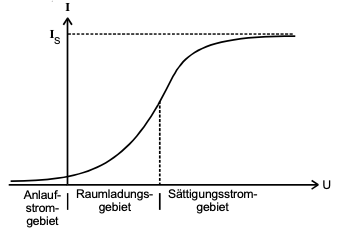
\includegraphics[width=0.7\textwidth]{content/Bilder/Kennlinie.png}
  \caption{Kennlinie einer Hochvakuum-Diode Q\cite{anleitungV504}.}
  \label{fig:Kennlinie}
\end{figure}
Das Anlaufstromgebiet ist durch einen exponentiellen Zusammenhang von dem Strom $I$ und des Potentials $V$ beschrieben. Dieser lautet
\begin{equation}
    j(V)=j_0 \exp \left( -\frac{e_0 \phi_{\text{A}}+e_0V}{k_{\text{B}T}}\right) = \text{const}\,\exp \left(-\frac{e_0V}{k_{\text{B}}T}\right)\,.
    \label{eqn:Anlaufstrom}
\end{equation}
Der Anlaufstrom bezeichnet den geringen Strom, gegen welche die Elektronen beim Verlassen der Kathode anlaufen können. Dies ist möglich, da die Energie dieser Elektronen
größer als die Austrittsarbeit $\phi_{\text{A}}$ ist. Das Raumladungsgebiet wird durch das Langmuir-Schottkyschen-Raumladungsgesetz 
\begin{equation}
    j = \frac{4}{9}\varepsilon_0 \sqrt{2 \frac{e_0}{m_0}}\frac{V^{\sfrac{3}{2}}}{a^2}
    \label{eqn:Raumladungsgesetz}
\end{equation}
beschrieben. In dem Raumladungsgebiet werden nicht alle emittierten Elektronen vom Anodenfeld erfasst, wodurch der gemessene Diodenstrom kleiner als der Sättigugnsstrom ist. 
Hierbei ist die Geschwindigkeit der Elektronen nicht konstant und die Raumladugnsdichte $\rho$ der Elektronen nimmt zur Anhode hin ab. 
Da die Raumladugnsdichte den Verlauf der Feldstärke zwischen der Anode und Kathode beschreibt, reichen die Feldlinien, die von der Anode ausgehen, nicht mehr vollständig bis zur Kathode.
Zuletzt ist in der Kennlinie der Sättigungsstromgebiet gekennzeichnet, der in \ref{sec:Sättigungsstromdichte} erläutert wird. Mithilfe von Ausschnitten der Kennlinie können die Kathodentemperatur $T$ sowie
die Austrittsarbeit der Kathode bestimmt werden.\\
Die Kathodentemperatur kann mithilfe aus der Leistungsbilanz des Heizstromfadens berechnet werden. Hier lautet die zugeführte Leistung lautet $N_{\text{zu}}=V_{\text{f}} I_{\text{f}}$.
Diese wird über Wärmestrahlung und Wärmeleitung der Fadenhalterung wieder abgegeben. Hier kann für die Wärmeleitung zu $N_{\text{WL}}=0,9 - 1\,\unit{\watt}$ abgeschätzt werden. Nach dem Stefan-Boltzmannschen Gesetzt ergibt sich für die
Strahlungsleistung $N_{\text{W}} = f\eta \sigma T^4$, wobei $\sigma = 5,7 \cdot 10^{-12}\,\sfrac{\unit{\watt}}{\unit{\centi\metre^2 \kelvin ^4}}$ gilt. $f$ ist die emittierende Kathodenoberfläche und $\eta =0,28$ der Emissionsgrad der Oberfläche.
Aus dem Energiesatz ergibt sich 
\begin{equation}
    I_{\text{f}}U_{\text{f}} = f \eta \sigma T^4 + N_{\text{WL}}\,.
    \label{eqn:aufWunschvonAmelie}
\end{equation}
